\documentclass[a4paper,11pt]{article} % Класс документа

% Подключаем полезные пакеты
\usepackage{booktabs}  % для \toprule, \midrule, \bottomrule
\usepackage{caption}   % улучшает внешний вид подписей
\usepackage{geometry}          % Настройка полей
\geometry{margin=2cm}
\usepackage{microtype}          % Улучшенный перенос слов
\usepackage{fontspec}         % Поддержка OpenType шрифтов
\usepackage[english,russian]{babel}  % Переносы для русского
\babelprovide[hyphenrules=russian]{russian}
\setmainfont{DejaVu Serif}
\setsansfont{DejaVu Sans}
\setmonofont{DejaVu Sans Mono}
\usepackage{amsmath, amssymb}  % Математика
\usepackage{graphicx}          % Для вставки изображений
\usepackage{hyperref}          % Ссылки и кликабельные URL
\usepackage{placeins}          % Для управления размещением плавающих объектов (FloatBarrier)
\usepackage{geometry}          % Настройка полей
\usepackage{circuitikz}        % Электрические схемы

\usepackage{titlesec}
\titleclass{\subsubsubsection}{straight}[\subsubsection]

\newcounter{subsubsubsection}[subsubsection]
\renewcommand\thesubsubsubsection{\thesubsubsection.\arabic{subsubsubsection}}

\titleformat{\subsubsubsection}
  {\normalfont\normalsize\bfseries}
  {\thesubsubsubsection}{1em}{}

\titlespacing*{\subsubsubsection}{0pt}{3.25ex plus 1ex}{1.5ex plus .2ex}

\setcounter{secnumdepth}{4}
\setcounter{tocdepth}{4}

\title{Ультразвуковая локальная навигация}
\author{Смирнов Егор Ильич}
\date{}

\begin{document}

\maketitle % Заголовок статьи

\section{Введение}
Надёжная локальная навигация является одним из ключевых условий безопасной и устойчивой работы беспилотных летательных
  аппаратов в стеснённых пространствах и в условиях ухудшенного или отсутствующего приёма сигналов глобальных
  навигационных спутниковых систем (GNSS/ГЛОНАСС). Даже в случае привязного летательного аппарта, когда полёт 
  механически ограничен тросом, задача точного и быстрого определения координат остаётся критичной: 
  она необходима для стабилизации и компенсации внешних возмущений (ветер, натяжение троса), 
  а также для реализации режимов удержания позиции и сопровождения объектов. Это особенно важно для БПЛА,
  несущих на себе телекоммуникационное оборудование. Область покрытия и возможность передачи сигнала напрямую\
  зависят от положения летательного аппарата.

На практике применяются различные подходы к локализации БПЛА. Спутниковая навигация
 (GNSS, включая дифференциальные и RTK-решения) обеспечивает абсолютные координаты на открытой местности,
  однако её точность и доступность существенно снижаются вблизи сооружений, в условиях загрязненного эфира, 
  внутри помещений и в городской застройке. 
  Визуальные методы (оптический поток, визуальная одометрия,
  визуально-инерциальные системы) способны обеспечивать высокую точность, однако зависят от освещённости, текстуры сцены
  и динамики окружающей среды; кроме того, они, как правило, требуют значительных вычислительных ресурсов.
  Лидарная одометрия отличается хорошей информативностью, однако сильно зависима от погодных условий.
  Инфраструктурные системы захвата движения (motion capture) 
  обеспечивают выдающуюся точность, но применимы только в специально оборудованных зонах и дорогостоящи в развёртывании.

Ультразвуковая навигация представляет собой привлекательный вариант для задач ближнего радиуса действия 
благодаря низкой стоимости, малому энергопотреблению и доступности компактных излучателей и приёмников. 
В таких системах положение объекта оценивается по времени распространения акустического сигнала между передатчиками 
и приёмниками с последующим пересчётом временных измерений в расстояния на основе величины скорости звука.
В зависимости от архитектуры могут применяться схемы измерения времени пролёта (ToF --- от англ. \textit{Time of Flight}),
разности времён прихода (TDoA --- от англ. \textit{Time Difference of Arrival})
или их комбинации с геометрическими методами триангуляции/мультилатерации.
В отличие от чисто бортовых методов измерения, ультразвуковые системы позволяют опираться на внешние маяки
и могут сохранять работоспособность даже в тех условиях, где оптика даёт сбои.
Вместе с тем ультразвуковое позиционирование имеет ограничения:
сравнительно малую дальность и отражения сигнала от поверхностей.

В настоящей работе рассматривается задача локальной навигации привязного БПЛА относительно платформы 
(в том числе потенциально подвижной) с использованием ультразвуковых измерений в качестве основного источника 
координатной информации.

\section{Описание системы}
Рассматриваемая система состоит из привязного БПЛА и наземной платформы, на которой размещается ультразвуковая
опорная подсистема. Платформа может быть стационарной или мобильной, поэтому все измерения и вычисления выполняются
в системе координат, связанной с платформой, а при необходимости, учитываются её наклоны.

В базовой конфигурации на платформе устанавливаются несколько ультразвуковых опорных узлов (далее --- якоря),
разнесённых на максимально возможное расстояние друг от друга. Геометрия якорей считается известной: координаты
каждого якоря заранее задаются в системе координат платформы. На БПЛА размещается ответная часть --- ультразвуковой
излучатель или приёмник (в зависимости от выбранной архитектуры), ориентированный в сторону платформы и работающий
в зоне прямой видимости опорных узлов.

\begin{figure}[h!]
    \centering
    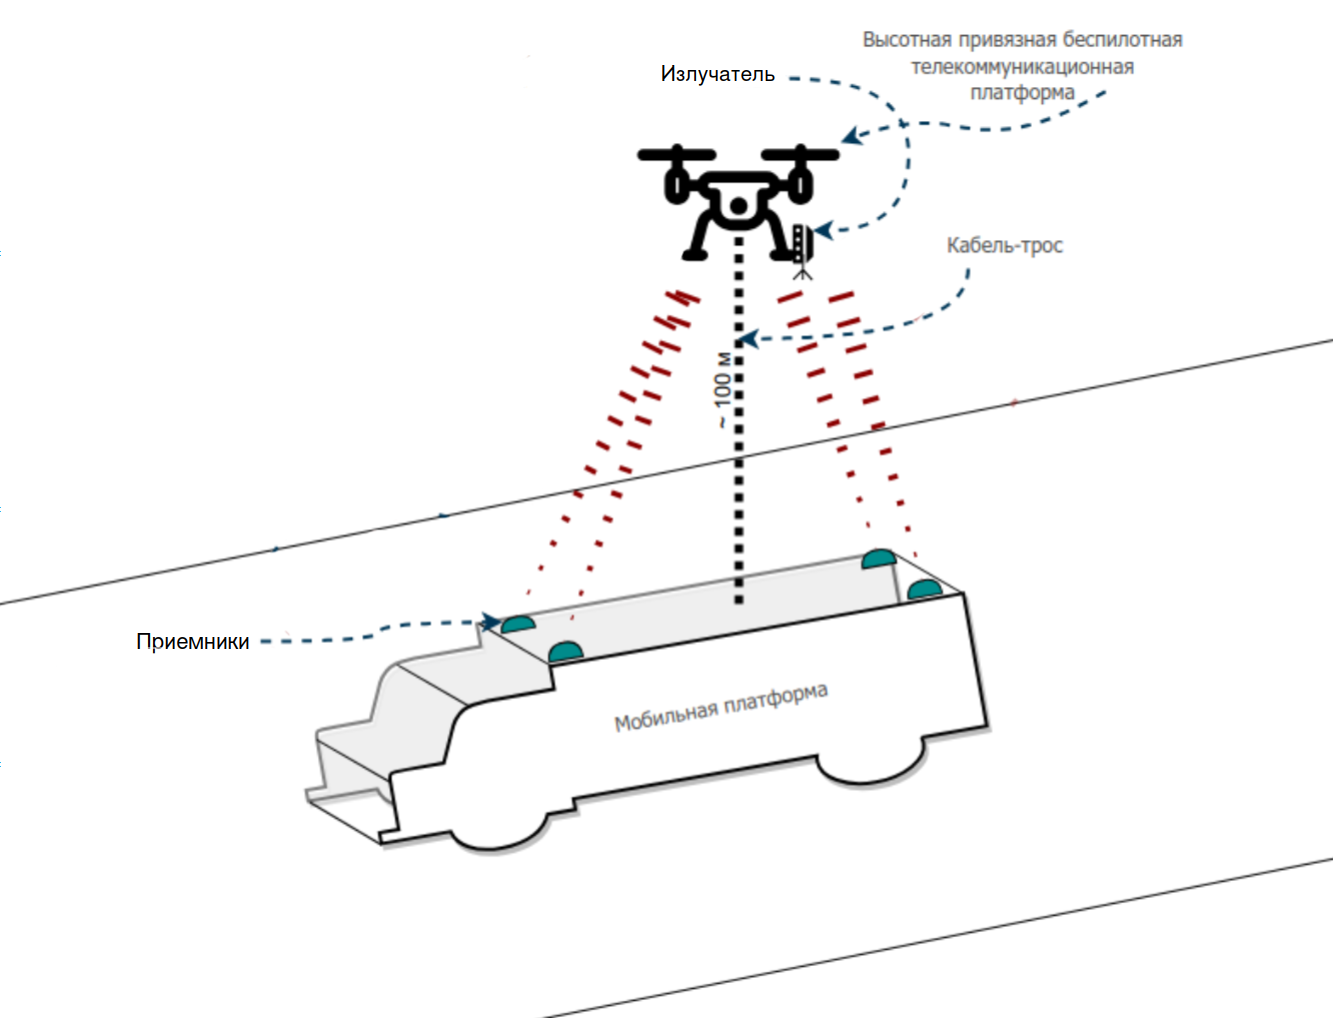
\includegraphics[width=0.9\textwidth]{images/system.png}
    \caption{Общая схема системы локальной навигации привязного БПЛА относительно платформы}
    \label{fig:system-overview}
\end{figure}

Принцип работы системы следующий. Опорные узлы на платформе и бортовой узел на БПЛА формируют набор измерений
времени распространения акустических импульсов. По измеренным временам вычисляются расстояния
до якорей, после чего координаты БПЛА определяются методом трилатерации в системе координат
платформы.

Для получения корректных расстояний требуется синхронизация времени между передающей и принимающей сторонами.
В привязном варианте синхронизирующий сигнал может быть передан по кабелю-тросу; альтернативно возможна
радиосинхронизация.

Если платформа подвержена наклонам, на ней размещается инерциальный датчик (например, акселерометр/IMU),
позволяющий оценивать ориентацию платформы относительно горизонта и, при необходимости, пересчитывать координаты
из платформенной системы координат в требуемую внешнюю систему отсчёта.

\section{Математическое описание системы}
\subsection{Максимальная дальность работы}
Под дальностью работы нужно понимать максимальное расстояние между излечателем и приемником, 
при котором приемник может стабильно детектировать сигнал. \\
Это расстояние зависит от нескольких факторов:


\begin{itemize}
  \item Мощность излучателя
  \item Чувствительность приемника
  \item Уровень шума в среде 
  \item Затухание звукового сигнала в среде
\end{itemize}
Остановимся подробнее на затухании звука.

Интенсивность звука убывает с расстоянием как:

\begin{equation}
 I(x) = I_0e^{-\alpha x}
\end{equation}
$\alpha$ — коэффициент затухания, дБ/м \\
\\
Согласно стандарту ISO 9613-1:1993~\cite{iso9613} , коэффициент затухания рассчитывается по формуле:

\begin{equation}\label{iso}
\alpha = 8.686 \cdot f^{2} \cdot \left[ 1.84 \cdot 10^{-11} \cdot \frac{p_r}{p_a} \cdot \left(\frac{T}{T_r}\right)^{0.5} + \left(\frac{T}{T_r}\right)^{-2.5} \cdot \left( \frac{0.01275 \cdot e^{-2239.1/T}}{f_{r,O} + \frac{f^{2}}{f_{r,O}}} + \frac{0.1068 \cdot e^{-3352.0/T}}{f_{r,N} + \frac{f^{2}}{f_{r,N}}} \right) \right]
\end{equation}

где:
\begin{itemize}
\item $\alpha$ — коэффициент затухания, дБ/м;
\item $f$ — частота звука, Гц;
\item $p_a$ — атмосферное давление, кПа;
\item $p_r = 101.325$ кПа — опорное давление;
\item $T$ — температура воздуха, К;
\item $T_r = 293.15$ К — опорная температура;
\item $f_{r,O}$ — частота релаксации кислорода, Гц;
\item $f_{r,N}$ — частота релаксации азота, Гц.
\end{itemize}

Частоты релаксации рассчитываются по формулам:

\begin{equation}
f_{r,O} = \frac{p_a}{p_r} \left( 24 + 4.04 \cdot 10^{4} h \frac{0.02 + h}{0.391 + h} \right)
\end{equation}

\begin{equation}
f_{r,N} = \frac{p_a}{p_r} \left( \frac{T}{T_r} \right)^{-1/2} \left( 9 + 280 \cdot h \cdot \exp \left( -4.170 \left[ \left(\frac{T}{T_r}\right)^{-1/3} - 1 \right] \right) \right)
\end{equation}

где $h$ — молярная концентрация водяного пара:
\begin{equation}
h = h_r \cdot \frac{p_{sat}}{p_a}
\end{equation}

Здесь $h_r$ — относительная влажность, $p_{sat}$ — давление насыщенного пара, которое рассчитывается по формуле:
\begin{equation}
p_{sat} = p_r \cdot 10^{-6.8346 \cdot \left( \frac{T_{01}}{T} \right)^{1.261} + 4.6151}
\end{equation}

где $T_{01} = 273.16$ К — температура тройной точки воды.
\\ 

По формуле \eqref{iso} видно, что коэффициент затухания прямо пропорционален квадрату частоты $f$.
Поэтому для обеспечения максимальной дальности частоты необходимо выбирать как можно ниже. \\

Для текущей системы была выбрана частота 25 кГц, она достаточно низкая для обеспечения дальности и при этом
находится вне слышимого диапазона.
\\
\\
Расчеты для этой частоты показали максимальное расстояние 35.6 метров.\\
Вычисления производились при следующих параметрах:
\begin{itemize}
\item относительная влажность --- $50\%$
\item температура воздуха --- $20\,^\circ\mathrm{C}$
\item мощность УК излучателя --- $105$~дБ (SPL --- Sound Pressure Level, на расстоянии 1~м от источника)
\item чувствительность УК приёмника --- $-95$~дБ
\end{itemize}

Следует отметить, что приведённая оценка является приблизительной; реальная дальность существенно зависит от конкретной реализации системы и внешних условий.

\subsection{Точность измерений расстояния}
Расстояние от БПЛА до якоря измеряется следующим образом: в известный момент времени излучатель
на БПЛА испускает сигнал. Спустя некоторое время приёмник на якоре его детектирует.
Так как микроконтроллеры на излучателе и приёмнике синхронизированы, время, которое потребовалось
для передачи сигнала, известно. Умножив его на скорость звука, получим искомое расстояние.

Значение мы будем получать с определенной погрешностью, разобьем ее на части (Рис \ref{fig:bias-variance})

\begin{figure}[h!]
  \centering
  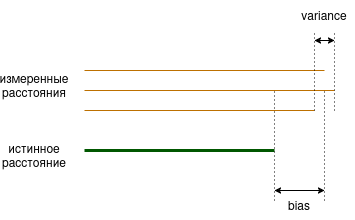
\includegraphics[width=0.7\textwidth]{images/bias-variance.png}
  \caption{Ошибка при определении расстояния}
  \label{fig:bias-variance}
\end{figure}

\subsubsection{Скорость звука}

Для определения расстояния нам необходимо знать скорость звука. Именно ошибка при вычислении скорости
вызывает систематическую ошибку в определении расстояний.
\\

Скорость звука $c$ в газе является термодинамической величиной. Для влажного воздуха в приближении идеальной
газовой смеси её можно оценить по выражению
\begin{subequations}\label{eq:speed-of-sound-humid-air} 
\begin{align}
  c &= \sqrt{\gamma\,R_{\mathrm{mix}}\,T}, \\
  R_{\mathrm{mix}} &= \frac{R}{M_{\mathrm{mix}}}, \\
  M_{\mathrm{mix}} &= (1-x_v)\,M_d + x_v\,M_v, \\
  x_v &= \frac{p_v}{p}, \\
  p_v &= h\,p_{\mathrm{sat}}(T), \\
  p_{\mathrm{sat}}(T) &= 611.21\,\exp\!\left(\frac{17.502\,(T-273.15)}{T-32.19}\right), \\
  \gamma &= \frac{c_{p,\mathrm{mix}}}{c_{v,\mathrm{mix}}}
  = \frac{c_{p,\mathrm{mix}}}{c_{p,\mathrm{mix}} - R_{\mathrm{mix}}}, \\
  c_{p,\mathrm{mix}} &= (1-x_v)\,c_{p,d}(T) + x_v\,c_{p,v}(T).
\end{align}
\end{subequations}
Выражения~\eqref{eq:speed-of-sound-humid-air} основаны на работе~\cite{cramer1993}.
Здесь $p_{\mathrm{sat}}(T)$ вычисляется по формуле Тетенса, применимой в диапазоне $-20\ldots 50~^\circ\mathrm{C}$.

После подстановки всех промежуточных величин в~\eqref{eq:speed-of-sound-humid-air} получается явное
выражение $c$ как функции трёх измеряемых параметров $(T, p, h)$:
\begin{equation}\label{eq:speed-of-sound-explicit}
  c(T,p,h) = \sqrt{\frac{c_{p,\mathrm{mix}}(T,p,h)\,R\,T}
                        {M_{\mathrm{mix}}(T,p,h)\bigl[c_{p,\mathrm{mix}}(T,p,h) - R/M_{\mathrm{mix}}(T,p,h)\bigr]}},
\end{equation}
где мольная доля пара и производные от неё величины имеют вид
\begin{align*}
  x_v(T,p,h)            &= \frac{h\,p_{\mathrm{sat}}(T)}{p}, \\
  M_{\mathrm{mix}}(T,p,h) &= M_d + x_v(T,p,h)\,(M_v - M_d), \\
  c_{p,\mathrm{mix}}(T,p,h) &= c_{p,d} + x_v(T,p,h)\,(c_{p,v} - c_{p,d}).
  c_{p,d} \approx 1005~\mathrm{J/(kg\cdot K)},\qquad
  c_{p,v} \approx 1850~\mathrm{J/(kg\cdot K)}.
\end{align*}

Обозначения, используемые в \eqref{eq:speed-of-sound-humid-air}, приведены в табл.~\ref{tab:speed-of-sound-notation}.

\begin{table}[!htbp]
  \centering
  \caption{Обозначения в модели скорости звука во влажном воздухе}
  \label{tab:speed-of-sound-notation}
  \small
  \begin{tabular}{lll}
    \toprule
    Обозначение & Значение & Единицы \\
    \midrule
    $c$ & скорость звука & м/с \\
    $T$ & абсолютная температура & $\mathrm{K}$ \\
    $p$ & общее давление & $\mathrm{Pa}$ \\
    $h$ & относительная влажность ($0\ldots 1$) & -- \\
    $x_v$ & мольная доля водяного пара & -- \\
    $p_v$ & парциальное давление пара & $\mathrm{Pa}$ \\
    $p_{\mathrm{sat}}(T)$ & давление насыщенного пара & $\mathrm{Pa}$ \\
    $R$ & универсальная газовая постоянная ($8.314462618$) & $\mathrm{J/(mol\cdot K)}$ \\
    $M_d$ & молярная масса сухого воздуха ($0.0289652$) & $\mathrm{kg/mol}$ \\
    $M_v$ & молярная масса воды ($0.01801528$) & $\mathrm{kg/mol}$ \\
    $M_{\mathrm{mix}}$ & молярная масса смеси & $\mathrm{kg/mol}$ \\
    $R_{\mathrm{mix}}$ & удельная газовая постоянная смеси & $\mathrm{J/(kg\cdot K)}$ \\
    $c_{p,d}(T)$ & теплоёмкость сухого воздуха при $p=\mathrm{const}$ & $\mathrm{J/(kg\cdot K)}$ \\
    $c_{p,v}(T)$ & теплоёмкость водяного пара при $p=\mathrm{const}$ & $\mathrm{J/(kg\cdot K)}$ \\
    $c_{p,\mathrm{mix}}$ & теплоёмкость смеси при $p=\mathrm{const}$ & $\mathrm{J/(kg\cdot K)}$ \\
    $c_{v,\mathrm{mix}}$ & теплоёмкость смеси при $V=\mathrm{const}$ & $\mathrm{J/(kg\cdot K)}$ \\
    $\gamma$ & показатель адиабаты смеси & -- \\
    \bottomrule
  \end{tabular}
\end{table}
\FloatBarrier

\textbf{Погрешность измерения параметров среды.}
Для расчёта скорости звука по формулам \eqref{eq:speed-of-sound-humid-air} требуются значения температуры $T$, давления $p$ и относительной влажности $h$. В реальной системе эти параметры измеряются датчиками, что вносит дополнительную погрешность в определение скорости звука.

В качестве датчика рассмотрим:
\begin{itemize}
    \item \textbf{BME280} (температура, давление, влажность): погрешность температуры $\pm 0.5\ ^\circ\mathrm{C}$, погрешность давления $\pm 1.2\ \mathrm{hPa}$ ($\pm 120\ \mathrm{Pa}$), погрешность влажности $\pm 3\%$.
\end{itemize}

\textbf{Погрешность модели.}
Погрешность модели $\Delta_{\text{мод}}$ определяется совокупностью приближений, использованных при выводе формул \eqref{eq:speed-of-sound-humid-air}. Рассмотрим составляющие:

\begin{enumerate}
    \item \textbf{Приближение идеального газа.} Уравнения \eqref{eq:speed-of-sound-humid-air} основаны на модели идеального газа.
    Реальные свойства воздуха описываются вторыми вириальными коэффициентами. Согласно анализу Cramer~\cite{cramer1993}, 
    учёт нелинейности уравнения состояния вносит поправку порядка $10^{-4}$ ($\sim 0.03$~м/с). Принимаем $\Delta_{\text{ид}} \approx 0.05$~м/с с запасом.
    
    \item \textbf{Упрощение теплоёмкостей.} В формулах \eqref{eq:speed-of-sound-humid-air} теплоёмкости $c_{p,d}$ и $c_{p,v}$ 
    принимаются постоянными. На самом деле они зависят от температуры. При изменении температуры от 0 до $40\ ^\circ\mathrm{C}$ 
    относительное изменение $c_{p,d}$ составляет около $0.1\%$, что даёт погрешность скорости звука $\Delta_{\text{cp}} \approx 0.3$~м/с.
  
    \item \textbf{Формула Тетенса.} Для расчёта давления насыщенного пара $p_{\mathrm{sat}}(T)$ используется формула Тетенса, 
    применимая в диапазоне $-20\ldots 50\ ^\circ\mathrm{C}$ с относительной погрешностью менее $0.5\%$. 
    Влияние на скорость звука незначительно: $\Delta_{\text{Тетенс}} \approx 0.01$~м/с.
    
    \item \textbf{Физические константы.} Универсальная газовая постоянная $R$ и молярные массы $M_d$, $M_v$ известны 
    с точностью лучше $10^{-5}$ (CODATA), их вклад пренебрежимо мал.
\end{enumerate}


Полная погрешность модели по закону накопления погрешностей:
\begin{equation}\label{eq:model-error}
    \Delta_{\text{мод}} = \sqrt{\Delta_{\text{ид}}^2 + \Delta_{\text{cp}}^2 + \Delta_{\text{Тетенс}}^2} = \sqrt{0.05^2 + 0.30^2 + 0.01^2} \approx 0.31\ \mathrm{m/s}.
\end{equation}

\textbf{Полная погрешность скорости звука.}
Погрешность определения $c$ складывается из погрешностей измерения параметров и погрешности модели:
\begin{equation}\label{eq:error-propagation}
    \Delta c = \sqrt{\left(\frac{\partial c}{\partial T}\Delta T\right)^2 + \left(\frac{\partial c}{\partial p}\Delta p\right)^2 + \left(\frac{\partial c}{\partial h}\Delta h\right)^2 + \Delta_{\text{мод}}^2}.
\end{equation}

Для оценки частных производных при околонормальных условиях ($T \approx 293\ \mathrm{K}$, $p \approx 101325\ \mathrm{Pa}$, $h \approx 0.5$) получаем:
\begin{align}
    \frac{\partial c}{\partial T} &\approx 0.60\ \mathrm{m/(s\cdot K)}, \\
    \frac{\partial c}{\partial p} &\approx -4.7 \cdot 10^{-4}\ \mathrm{m/(s\cdot Pa)}, \\
    \frac{\partial c}{\partial h} &\approx 0.08\ \mathrm{m/s}.
\end{align}

Подставляя погрешности датчиков BME280 ($\Delta T = 0.5\ \mathrm{K}$, $\Delta p = 120\ \mathrm{Pa}$, $\Delta h = 0.03$) и $\Delta_{\text{мод}} = 0.31$~м/с:
\begin{align}
    \Delta c_T &= 0.60 \cdot 0.5 = 0.30\ \mathrm{m/s}, \\
    \Delta c_p &= 4.7 \cdot 10^{-4} \cdot 120 \approx 0.06\ \mathrm{m/s}, \\
    \Delta c_h &= 0.08 \cdot 0.03 \approx 0.002\ \mathrm{m/s}.
\end{align}

Полная погрешность:
\begin{equation}
    \Delta c = \sqrt{0.30^2 + 0.06^2 + 0.002^2 + 0.31^2} \approx \sqrt{0.186} \approx 0.43\ \mathrm{m/s}.
\end{equation}

Таким образом, при использовании датчиков среднего класса точности полная погрешность определения скорости звука составляет около $\pm 0.43\ \mathrm{m/s}$ ($\sim \pm 0.13\%$). Основной вклад вносят погрешность измерения температуры ($\sim 70\%$) и погрешность модели ($\sim 52\%$); влияние давления и влажности значительно меньше.
\\

\textbf{Проверка по табличным данным.}
Для верификации оценки погрешности модели выполним сравнение расчётного значения скорости звука с табличными данными при стандартных условиях (сухой воздух, $T = 273.15$~K, $p = 101325$~Па, $h = 0$).

По формулам \eqref{eq:speed-of-sound-humid-air} при $h = 0$ получаем $x_v = 0$, $M_{\text{mix}} = M_d$, $R_{\text{mix}} = R/M_d$, $\gamma = c_{p,d}/(c_{p,d} - R_{\text{mix}})$, откуда
\begin{equation}
    c_{\text{расч}} = \sqrt{\gamma \frac{R}{M_d} T} = \sqrt{1.402 \cdot \frac{8.314}{0.028965} \cdot 273.15} \approx 331.3\ \mathrm{m/s}.
\end{equation}

Табличное значение скорости звука в сухом воздухе при $0\ ^\circ\mathrm{C}$ и нормальном атмосферном давлении согласно \cite{iso2533} составляет $c_{\text{табл}} = 331.29$~м/с. Разница между расчётным и табличным значениями:
\begin{equation}
    \Delta c_{\text{проверка}} = |c_{\text{расч}} - c_{\text{табл}}| \approx |331.3 - 331.29| = 0.01\ \mathrm{m/s}.
\end{equation}

Полученное расхождение ($\sim 0.003\%$) значительно меньше оценённой погрешности модели $\Delta_{\text{мод}} \approx 0.31$~м/с, что подтверждает корректность оценки с запасом. Разница объясняется округлениями констант в расчёте и не учтённым влиянием реальных свойств газа (вторые вириальные коэффициенты), которое как раз и даёт основной вклад в $\Delta_{\text{мод}}$.
\\

\textbf{Выводы.}
Проведённый анализ показал, что при использовании недорогих датчиков типа BME280 основная погрешность определения скорости звука ($\sim 0.43$~м/с) определяется погрешностью измерения температуры ($0.30$~м/с) и погрешностью модели ($0.31$~м/с). Проверка по табличным данным подтвердила, что оценка погрешности модели является консервативной (завышенной), что приемлемо для инженерных расчётов.


\subsubsection{Точность измерений времени}
Микроконтроллер измеряет время, которое потребовалось сигналу, чтобы долететь от излучателя до приемника.
Он это делает дискретно, следовательно всегда будет существовать погрешность $\Delta t$.

Ошибка измерений расстояния будет соответсвенно:
\begin{equation}
 \pm d = \frac{c}{2 \Delta t}
\end{equation}

Приведем характерные значения:

\begin{table}[h!]
    \centering
    \begin{tabular}{|c|c|}
        \hline
        $\Delta t$ & $d$ \\
        \hline
        1 мкс & 0.17 мм  \\
        10 мкс & 1.7 мм \\
        100 мкс & 17 мм \\
        1000 мкс & 17 см \\
        \hline
    \end{tabular}
    \label{tab:example}
\end{table}
Современные микроконтроллеры позволяют измерять время с точностью $\leq 10$~мкс, это даёт ошибку в 2~мм.
Именно эту ошибку мы называем случайной, она будет индивидуальной для каждого измерения.

\paragraph{Итоги\\}
\begin{itemize}
  \item Систематическая ошибка - 0.12 \%
  \item Случайная ошибка       -    2 мм
\end{itemize}


\subsubsection{Точность определения координат}

При трилатерации в трёхмерном пространстве точность определения координат зависит не только от точности измерения расстояний до якорей, но и от их геометрического расположения. Данный эффект описывается коэффициентом геометрического ослабления точности (GDOP — Geometric Dilution of Precision) \cite{kaplan2005,misra2006}.

Коэффициент GDOP характеризует влияние геометрии расположения якорей на распространение \textbf{случайных} ошибок измерения расстояний в ошибку оценки координат. В рамках линейной модели оценивания с нулевым средним ошибок измерений GDOP определяет ковариацию оценки координат. Систематические ошибки приводят к смещению оценки и не описываются коэффициентом GDOP \cite{kay1993,hayes1996}.

\textbf{Постановка задачи.} Рассмотрим четыре якоря, расположенные в вершинах квадрата в плоскости $z=0$:
$$
A_1(+a/2, +a/2, 0), \quad A_2(-a/2, +a/2, 0), \quad A_3(-a/2, -a/2, 0), \quad A_4(+a/2, -a/2, 0).
$$

Объект находится в точке $P(0, 0, H)$ на высоте $H$ над центром квадрата. Измеренные расстояния до якорей:
$$
d_i = \sqrt{(x-x_i)^2 + (y-y_i)^2 + (z-z_i)^2} + \varepsilon_i,
$$
где $\varepsilon_i$ — случайная ошибка измерения с дисперсией $\sigma_d^2$.
\\

\textbf{Матрица Якоби.} Линеаризуем уравнения в окрестности истинной позиции. Пусть $D = \sqrt{a^2/2 + H^2}$ — расстояние от объекта до каждого якоря. Матрица Якоби имеет вид:
$$
J =
\begin{pmatrix}
+\frac{a}{2D} & +\frac{a}{2D} & -\frac{H}{D} \\
-\frac{a}{2D} & +\frac{a}{2D} & -\frac{H}{D} \\
-\frac{a}{2D} & -\frac{a}{2D} & -\frac{H}{D} \\
+\frac{a}{2D} & -\frac{a}{2D} & -\frac{H}{D}
\end{pmatrix}.
$$

\textbf{Вычисление $J^T J$.} Благодаря симметрии расположения якорей матрица $J^T J$ является диагональной:
$$
J^T J =
\begin{pmatrix}
\frac{a^2}{D^2} & 0 & 0 \\
0 & \frac{a^2}{D^2} & 0 \\
0 & 0 & \frac{4H^2}{D^2}
\end{pmatrix}.
$$

\textbf{Ковариационная матрица и GDOP.} В рамках метода наименьших квадратов ковариационная матрица оценки координат определяется выражением \cite{hayes1996,kay1993}:
$$
\Sigma = \sigma_d^2 (J^T J)^{-1}.
$$

Отсюда:
$$
\Sigma = \sigma_d^2
\begin{pmatrix}
\frac{D^2}{a^2} & 0 & 0 \\
0 & \frac{D^2}{a^2} & 0 \\
0 & 0 & \frac{D^2}{4H^2}
\end{pmatrix}.
$$

Среднеквадратичная ошибка положения (PDOP — Position Dilution of Precision) определяется как:
$$
\sigma_{xyz} = \sqrt{\mathrm{tr}(\Sigma)} = \sigma_d \sqrt{\frac{2D^2}{a^2} + \frac{D^2}{4H^2}}.
$$

Подставляя $D^2 = \frac{a^2}{2} + H^2$, получаем:
$$
\boxed{
\sigma_{xyz} = \sigma_d \cdot D \cdot \sqrt{\frac{2}{a^2} + \frac{1}{4H^2}}
}
$$

где:
\begin{itemize}
    \item $\sigma_{xyz}$ — среднеквадратичная ошибка положения, м;
    \item $\sigma_d$ — СКО измерения расстояния до якоря, м;
    \item $D = \sqrt{a^2/2 + H^2}$ — расстояние до якоря, м;
    \item $a$ — расстояние между якорями, м;
    \item $H$ — высота объекта, м.
\end{itemize}

На рис.~\ref{fig:gdop-anchor-distance} представлена зависимость ошибки позиционирования от взаимного расположения якорей при фиксированной ошибке измерения $\sigma_d = 2$ мм и расстоянии до якорей $D = 25$ м.

\begin{figure}[h!]
    \centering
    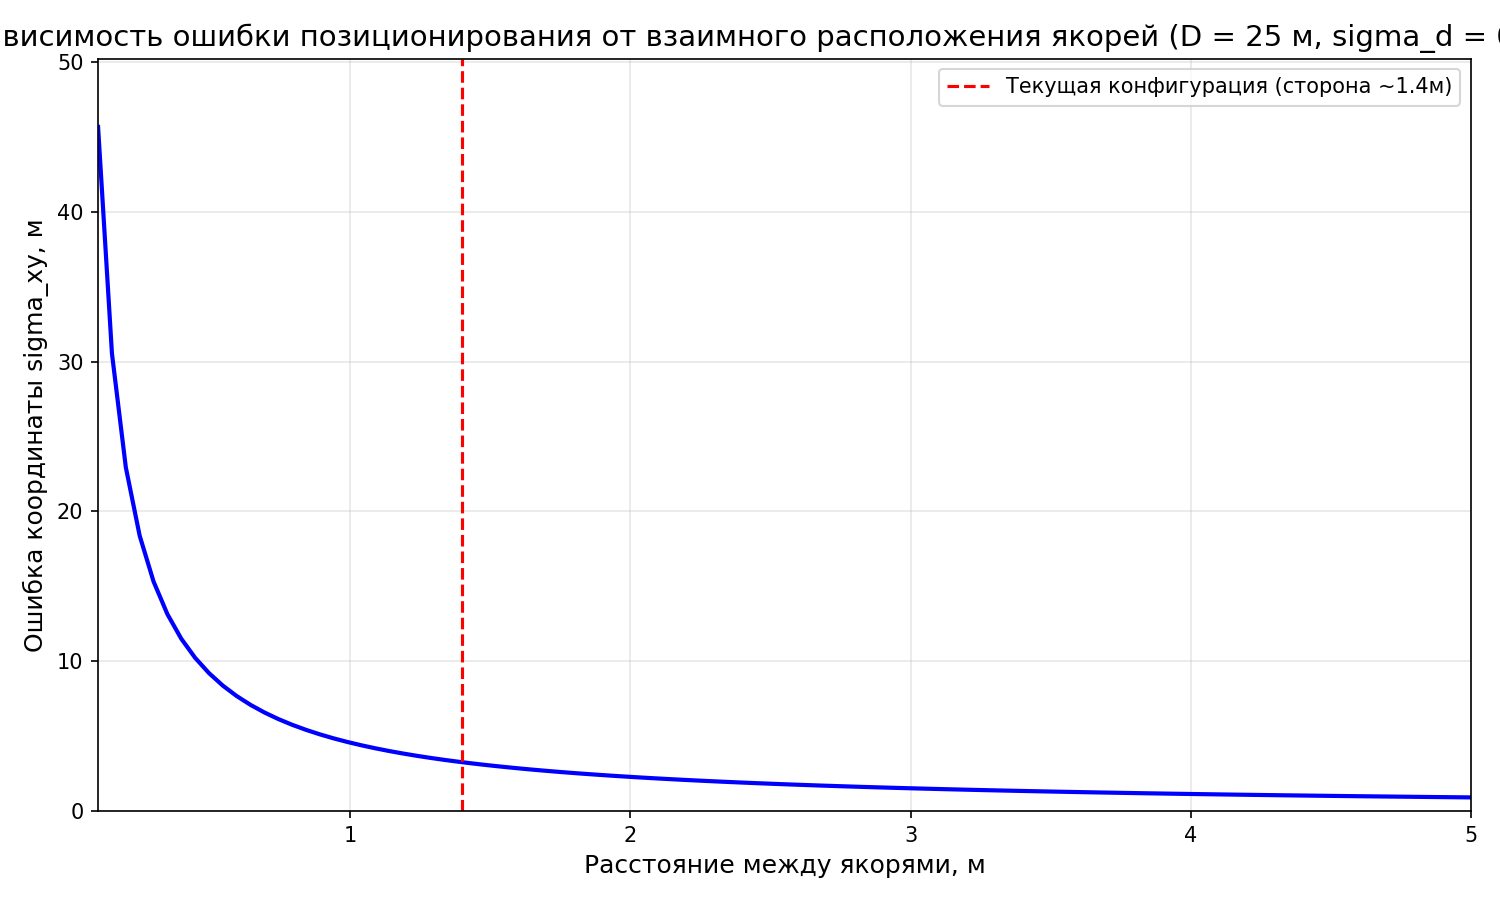
\includegraphics[width=1\textwidth]{images/gdop-vs-anchor-distance.png}
    \caption{Зависимость ошибки позиционирования от геометрии расположения якорей}
    \label{fig:gdop-anchor-distance}
\end{figure}

\paragraph{Оценка погрешности.}
Рассмотрим характерные параметры системы: высота объекта $H = 25$ м, расстояние между якорями $a = 2$ м. В этом случае:

\begin{itemize}
  \item систематическая ошибка измерения расстояния приводит к смещению оценки порядка $3$ см;
  \item случайная ошибка измерений с учётом эффекта GDOP приводит к СКО порядка $5$ см.
\end{itemize}

Таким образом, суммарная ошибка позиционирования в худшем случае может достигать порядка $8$ см.
\subsection{Методы решения задачи трилатерации}
Для получения координат БПЛА при известных расстояниях до якорей необходимо решить задачу трилатерации.
Для её решения в настоящей работе рассмотрены два метода: аналитический и вычислительный метод Гаусса-Ньютона. В экспериментах
были протестированы несколько вычислительных методов и все они дали идентичные результаты,
поэтому предпочтение отдано методу Гаусса-Ньютона ввиду его низкой вычислительной сложности.
\subsubsection{Аналитическое решение задачи трилатерации в пространстве по трём расстояниям}

Пусть заданы три опорные точки в плоскости \(z=0\):
\[
P_1 = (x_1, y_1, 0), \qquad
P_2 = (x_2, y_2, 0), \qquad
P_3 = (x_3, y_3, 0),
\]
и измеренные расстояния от неизвестной точки \(P=(x,y,z)\) до них:
\[
r_1,\; r_2,\; r_3.
\]

\subsubsubsection*{1. Уравнения сфер}

Координаты точки \(P\) удовлетворяют системе уравнений трёх сфер:
\[
(x - x_i)^2 + (y - y_i)^2 + z^2 = r_i^2, \qquad i = 1,2,3.
\]

\subsubsubsection*{2. Получение линейной системы для координат \(x\) и \(y\)}

Вычтем уравнения для \(i=2\) и \(i=3\) из уравнения для \(i=1\).  
Так как член \(z^2\) присутствует во всех трёх уравнениях, он сокращается. Получаем:

\begin{align}
2(x_2-x_1)x + 2(y_2-y_1)y &= r_1^2 - r_2^2 + x_2^2 - x_1^2 + y_2^2 - y_1^2, \\
2(x_3-x_1)x + 2(y_3-y_1)y &= r_1^2 - r_3^2 + x_3^2 - x_1^2 + y_3^2 - y_1^2.
\end{align}

В матричной форме:
\[
A
\begin{pmatrix} x \\ y \end{pmatrix}
=
\begin{pmatrix} b_1 \\ b_2 \end{pmatrix},
\]
где
\[
A =
\begin{pmatrix}
2(x_2-x_1) & 2(y_2-y_1) \\
2(x_3-x_1) & 2(y_3-y_1)
\end{pmatrix},
\]
\[
b_1 = r_1^2 - r_2^2 + x_2^2 - x_1^2 + y_2^2 - y_1^2,
\qquad
b_2 = r_1^2 - r_3^2 + x_3^2 - x_1^2 + y_3^2 - y_1^2.
\]

Если опорные точки не коллинеарны, то \(\det A \neq 0\), и система имеет единственное решение:
\[
\begin{pmatrix} x \\ y \end{pmatrix} = A^{-1} \begin{pmatrix} b_1 \\ b_2 \end{pmatrix}.
\]

\subsubsubsection*{3. Определение координаты \(z\)}

После нахождения \(x\) и \(y\) подставим их в первое уравнение сферы:
\[
z^2 = r_1^2 - (x - x_1)^2 - (y - y_1)^2.
\]

Отсюда:
\[
z = \pm\sqrt{\,r_1^2 - (x - x_1)^2 - (y - y_1)^2\,}.
\]

Если
\[
r_1^2 - (x - x_1)^2 - (y - y_1)^2 < 0,
\]
то система не имеет действительных решений (данные несовместны).

Поскольку сферы симметричны относительно плоскости \(z=0\), существует максимум два решения, соответствующие различным знакам корня.  
В данной задаче выбирается решение с положительной высотой:
\[
z > 0.
\]

\subsubsubsection*{4. Итоговое решение}

Искомая точка пересечения сфер:
\[
P = (x, y, z),
\]
где \((x,y)\) находятся из линейной системы
\[
A\begin{pmatrix}x\\y\end{pmatrix} = \begin{pmatrix}b_1\\b_2\end{pmatrix},
\]
а координата \(z\) определяется как
\[
z = \sqrt{\,r_1^2 - (x - x_1)^2 - (y - y_1)^2\,}.
\]

При этом берётся корень со знаком «плюс», так как требуется решение с \(z>0\).

\subsubsection{Метод Гаусса-Ньютона}

Этот метод используется для минимизации суммы квадратов, с учётом нашей задачи,
функция для минимизации будет выглядеть следующим образом:

\[
\boxed{%
\; \min_{\mathbf{p}}\; J(\mathbf{p}), \qquad
J(\mathbf{p}) = \sum_{i=1}^{N} w_i\bigl(\,\hat r_i - \|\mathbf{p}-\mathbf{a}_i\|\,\bigr)^2
}
\]

\begin{itemize}
  \item $\hat r_i$ \;— измеренное расстояние от якоря $i$ до объекта .
  \item $\mathbf{a}_i$ \;— вектор координат $i$-го якоря.
  \item $\mathbf{p}$ \;— вектор неизвестных координат объекта.
  \item $w_i$ \;— вес измерения $i$ (обычно обратный дисперсии).
  \item $J(\mathbf{p})$ \;— целевая функция суммы взвешенных квадратов невязок.
\end{itemize}

Подробное изложение метода выходит за рамки настоящей работы; его описание можно найти в~\cite{hayes1996}.
В качестве начального приближения целесообразно использовать предыдущую позицию БПЛА
или данные инерциальной навигационной системы: при хорошем начальном приближении метод
сходится за единичное число итераций, что обеспечивает низкие вычислительные затраты.

\subsubsection{Сравнительный анализ}
Для сравнения точности этих методов был проведён численный эксперимент в программе на Python.
\\
\paragraph{Постановка эксперимента\\}
Рассмотрим конфигурацию из 4 якорей, расположенных по углам квадрата с шириной 2 метра, далее
\begin{itemize}
    \item Выбираем случайные координаты БПЛА, примерно в 25 метрах над платформой
    \item Измеряем расстояния от обьекта до якорей
    \item Подмешиваем в расстояния систематическую и случайную ошибку
    \item Передаем расстояния в вычислительные методы и получаем результат.
    \item Вычисляем ошибку координат
\end{itemize}
Эксперимент с 5 якорями проводится аналогично, пятый якорь добавляется в центр квадрата.


Аналитический метод предполагает известные расстояния только до трех точек, поэтому мы будем вычилсять
координаты для каждой тройки точек в отдельности.

\begin{center}
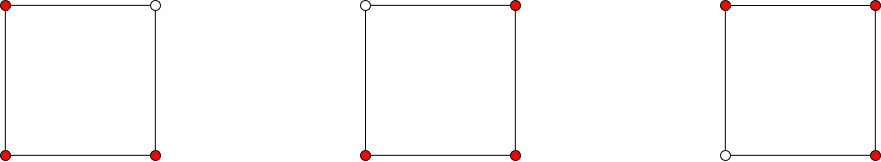
\includegraphics[width=1\textwidth]{images/triplet-selection.png}
    Рис.3 выбор троек точек
\end{center}
Далее полученные координаты усредняем по всем тройкам.
\\
\\
Вычислительный же метод работает следующим образом: в качестве начального прилижение будет браться
аналитическое решение по любой из троек, далее следуют итерации метода Гаусса-Ньютона, 
учитывающие расстояние до всех якорей.
\paragraph{Результаты\\}
Систематическая ошибка одинаково влияет на точность аналитического и вычислительного метода,
поэтому в экспериментах она имеет фиксированное значение в 0.12 \%.\\
Посмотрим на точность методов в зависимости от случайной ошибки:\\
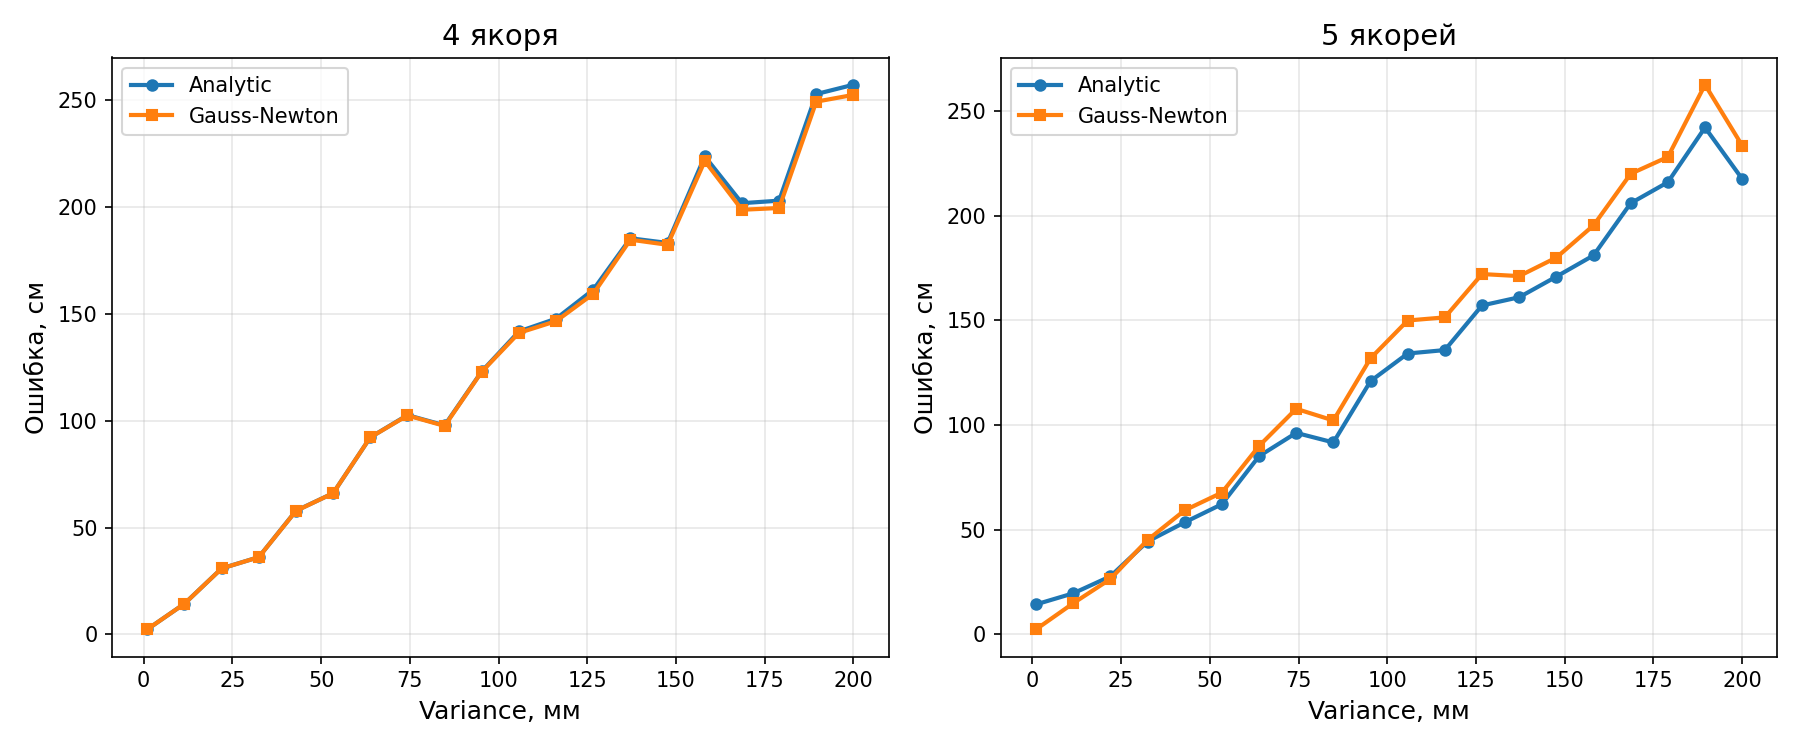
\includegraphics[width=1\textwidth]{images/error_vs_variance.png}
\\
каждая точка на графике соответсвует средней ошибке по 50 измеерениям.\\
\\
\begin{itemize}
  \item \textbf{4 якоря:} результаты почти одинаковые.
  \item \textbf{5 якорей:} аналитический метод показывает себя лучше при больших значениях ошибки, и хуже при малых.
Ухудшение точности на малых ошибках можно обьяснить тем, что в конфигурации из 5 якорей существуют тройки,
где якоря находятся ближе дрг к другу. Это повышает GDOP ошибку и ухудшает общий результат при усреднении.
\end{itemize}

В таблицах приведены средние значения ошибки по 1000 измерений, в зависимости от разных значений случайной ошибки 
\begin{table}[h!]
  \centering
  \begin{minipage}{0.48\textwidth}
    \centering
    \caption{Аналитический метод}
    \begin{tabular}{|c|c|c|}
        \hline
        $\sigma$, м & 4 якоря, см & 5 якорей, см \\
        \hline
        0.002 & 3.44 & 15.51 \\
        \hline
        0.005 & 6.98 & 16.56 \\
        \hline
        0.01 & 12.78 & 18.87 \\
        \hline
        0.05 & 62.52 & 57.98 \\
        \hline
        0.1 & 128.21 & 116.31 \\
        \hline
    \end{tabular}
  \end{minipage}%
  \hspace{0.04\textwidth}%
  \begin{minipage}{0.48\textwidth}
    \centering
    \caption{Метод Гаусса-Ньютона}
    \begin{tabular}{|c|c|c|}
        \hline
        $\sigma$, м & 4 якоря, см & 5 якорей, см \\
        \hline
        0.002 & 3.44 & 3.43 \\
        \hline
        0.005 & 6.83 & 6.69 \\
        \hline
        0.01 & 12.96 & 12.59 \\
        \hline
        0.05 & 62.68 & 62.58 \\
        \hline
        0.1 & 128.78 & 125.42 \\
        \hline
    \end{tabular}
  \end{minipage}
\end{table}

В нашей системе случайная ошибка имеет значение 0.002 метра, при этом полная ошибка позиционирования
в среднем не превышает 4 см, что полностью укладывается в теоритические оценки.

Аналитический метод вычислительно проще метода Гаусса-Ньютона, и оптимально будет использовать именно его,
на конфигурации из 4 якорей.

\section{Реализация}

\subsection{Узел БПЛА (передающая часть)}
\label{sec:uav-node}

Узел БПЛА выполняет две задачи: излучение пачек ультразвукового сигнала на частоте 25~кГц
с амплитудной OOK-модуляцией (\textit{On--Off Keying}~--- двухуровневая амплитудная
манипуляция, при которой биту~«1» соответствует наличие несущей, биту~«0»~--- её
отсутствие) и радиочастотную синхронизацию начала каждой пачки с центральным
узлом на платформе. Жёсткое совмещение моментов начала ультразвукового и радиоимпульса
является принципиальным требованием: при заданном уровне точности ToF на уровне миллиметра
рассогласование между фактическим стартом акустического сигнала и зафиксированным
радиосинхросигналом не должно превышать нескольких микросекунд.

\subsubsection{Структурная схема}

В состав узла входят микроконтроллер ESP32-WROOM-32, сверхширокополосный (UWB) радиомодуль
DWM1000 (Decawave/Qorvo), счетверённый аналоговый ключ SN74HC4066N, мостовой драйвер
TC4427A и пьезоизлучатель Murata MA40S4S (рис.~\ref{fig:uav-block}).
ESP32 формирует непрерывную несущую 25~кГц на одном из выводов LEDC и одновременно
конфигурирует DWM1000 по интерфейсу SPI. Открытие тракта несущей на драйвер выполняется
аппаратно сигналом EXTTXE радиомодуля.

\begin{figure}[h!]
\centering
\begin{tikzpicture}[
  blk/.style={draw, thick, rectangle, minimum width=2.6cm, minimum height=1.1cm,
              align=center, font=\small, inner sep=3pt},
  arr/.style={thick, ->}
]
\node[blk] (mcu)  at (0,    1.4) {ESP32\\[-2pt]{\scriptsize $A$, $B$: 25\,кГц + OOK}};
\node[blk] (rf)   at (0,   -1.4) {DWM1000\\[-2pt]{\scriptsize Delayed TX}};
\node[blk] (sw)   at (4.8,  0)   {SN74HC4066\\[-2pt]{\scriptsize 2 ключа: $A$, $B$}};
\node[blk] (drv)  at (8.8,  0)   {TC4427A\\[-2pt]{\scriptsize драйвер (мост)}};
\node[blk] (pz)   at (12.4, 0)   {MA40S4S};
\draw[arr] (mcu.east) -| (sw.north);
\draw[arr] (rf.east)  -| (sw.south);
\draw[arr] (sw) -- (drv);
\draw[arr] (drv) -- (pz);
\draw[<->, thick] (mcu.south) -- (rf.north) node[midway, right, font=\scriptsize] {SPI};
\node[font=\scriptsize] at (2.6,  1.0) {2 канала};
\node[font=\scriptsize] at (2.6, -1.0) {EXTTXE};
\end{tikzpicture}
\caption{Структурная схема узла БПЛА: ESP32 формирует два противофазных канала
несущей 25~кГц ($A$ и~$B$) для дифференциального возбуждения моста и управляет
радиомодулем DWM1000 по SPI; в момент старта UWB-пакета модуль аппаратно открывает
оба аналоговых ключа SN74HC4066 общим сигналом EXTTXE.}
\label{fig:uav-block}
\end{figure}

\subsubsection{Аппаратная синхронизация через EXTTXE}

Источники временной погрешности при синхронизации можно разделить на два принципиально
различных типа: случайный джиттер и фиксированную задержку. Эти величины по-разному
влияют на точность ToF, и схема построена так, чтобы исключить один и поглотить другой.

\textbf{Случайный джиттер (опасен).}
Программный запуск передачи в ESP32 проходит через прерывания операционной системы
FreeRTOS. Время реакции на прерывание зависит от состояния планировщика, кэшей
инструкций и обработчиков более приоритетных прерываний; результирующий разброс
момента старта составляет 1--5~мкс. Этот разброс непредсказуем и не воспроизводится
от пакета к пакету, поэтому он напрямую переходит в погрешность ToF: при $\Delta t = 1$~мкс
ошибка дальности $\Delta d = c\,\Delta t \approx 0{,}34$~мм. При требуемой точности
на уровне миллиметра такой джиттер недопустим.

\textbf{Фиксированная задержка (безопасна).}
Радиочастотной цепи DWM1000 от момента записи команды по SPI до фактического подъёма
сигнала EXTTXE требуется ${\sim}150$~мкс на инициализацию синтезатора и формирование
RF-преамбулы. Эта задержка определяется аппаратными свойствами микросхемы и постоянна
с точностью до субнаносекунд от пакета к пакету. На точность ToF она не влияет:
одинаковый сдвиг моментов на передающей и приёмной стороне сокращается при вычитании
разности времён, а постоянный остаток учитывается одной аддитивной константой,
определяемой при калибровке. Таким образом, важен не абсолютный момент старта,
а отсутствие случайной составляющей в нём.

\textbf{Решение.}
Применяется аппаратный механизм отложенной передачи DWM1000 (\textit{Delayed TX}).
ESP32 заранее, за несколько сотен микросекунд до требуемого момента, программирует
по SPI время старта; далее весь процесс ведёт встроенный радиочастотный таймер модуля
с шагом 15~пс. В заранее запрограммированный момент DWM1000 поднимает в высокий уровень
сигнал EXTTXE (вывод GPIO5, выведенный на внешние контакты модуля). Поскольку SPI-команда
подаётся заблаговременно, программный джиттер ESP32 укладывается в окно ожидания и
не переходит на момент EXTTXE; стартом командует только аппаратный таймер.

Сигнал EXTTXE подаётся на разрешающие входы аналоговых ключей SN74HC4066N.
Непрерывная несущая 25~кГц с выводов ESP32 попадает на драйвер только в активном
состоянии EXTTXE; до этого момента и после завершения пачки путь сигнала разорван.
Моменты физического начала ультразвукового излучения и UWB-передачи жёстко связаны
общим логическим фронтом; взаимный джиттер между ними определяется задержками
логических вентилей и не превышает 10~нс, что соответствует ошибке ToF
$\Delta d \approx 3{,}4$~мкм~--- пренебрежимо мало по сравнению с погрешностью
детектирования переднего фронта огибающей.

В начале каждой OOK-посылки формируется преамбула из нескольких пустых периодов несущей.
Её роль вспомогательная~--- дать времени отработать переходные процессы пьезопреобразователя
и приёмного тракта; информационные биты идут после преамбулы и потому не теряются.

\subsubsection{Управление мостом и активное гашение пьезоизлучателя}

Драйвер TC4427A построен по мостовой (полу-H) схеме и питает пьезопреобразователь
дифференциально, то есть напряжением между двумя своими выходами. Чтобы получить
двуполярное возбуждение, на оба входа драйвера приходят два сигнала с двух выводов
ESP32; во всё время передачи оба пути активны, поэтому в работе одновременно участвуют
оба ключа SN74HC4066N. Один ключ коммутирует первый сигнал ($A$) от ESP32 ко входу
$\text{IN}_A$ драйвера, второй~--- сигнал ($B$) ко входу $\text{IN}_B$. Общим
разрешающим сигналом для обоих ключей служит EXTTXE, что обеспечивает строго
одновременное открытие путей и сохраняет наносекундную привязку к UWB-пакету.

Кодирование OOK задаётся не коммутацией ключей, а соотношением фаз сигналов $A$ и $B$,
формируемых ESP32:
\begin{itemize}
    \item на бите~«1» $A$ и $B$ противофазны (сдвиг $180^\circ$): $\text{IN}_A$ и $\text{IN}_B$
          противоположны, выходы драйвера формируют дифференциальный размах
          ${\pm}V_\text{DD}$ на излучателе~--- передача несущей;
    \item на бите~«0» $A$ и $B$ совпадают (сдвиг $0^\circ$): $\text{IN}_A = \text{IN}_B$,
          оба выхода драйвера переключаются синхронно и в каждый момент находятся
          на одном уровне. Дифференциальное напряжение на излучателе равно нулю,
          а сам излучатель оказывается замкнут через нижние ключи моста с малым
          сопротивлением открытого канала ($R_{DS(\text{on})} \sim 0{,}5$~Ом).
\end{itemize}

Пьезоэлектрический преобразователь MA40S4S обладает высокой механической добротностью:
после прекращения возбуждения собственные колебания затухают за ${\sim}400$~мкс.
Без принудительного гашения это создаёт «мёртвую зону» после каждого переданного символа
и ухудшает разделение OOK-битов. В предложенной схеме на бите~«0» запасённая
в пьезопреобразователе механическая энергия диссипируется через мост на сопротивлении
$R_{DS(\text{on})}$, то есть гасится активно за время порядка одного периода несущей.

Управляющие входы двух неиспользуемых ключей микросхемы SN74HC4066N подтянуты к общему
проводу резисторами 10~кОм, гарантируя их закрытое состояние.

\FloatBarrier

\subsection{Узел якоря: обработка сигнала}

Цепь обработки сигнала каждого якоря включает четыре последовательных блока
(рис.~\ref{fig:anchor-block}): предусилитель~INA128P, усилитель~TL072CN
(два каскада: ФНЧ и ФВЧ) и демодулятор (детектор огибающей совместно с компаратором~LM311P).

Пьезоприёмник является механическим резонатором: любое акустическое воздействие ---
хлопок, удар, вибрация --- преобразуется в затухающие колебания на той же частоте~25~кГц,
что и полезный сигнал. Поэтому полосовой фильтр не позволяет отличить полезный сигнал
от механического шума. Надёжное распознавание обеспечивается временным кодированием:
передатчик излучает пачки длительностью~0{,}5--2~мс, а микроконтроллер идентифицирует
сигнал по временному шаблону. Фильтр выполняет вспомогательную роль: подавляет
электрические помехи в схеме (наводки питания, ВЧ-мусор), что позволяет поднять
коэффициент усиления без перегрузки.

\begin{figure}[h!]
\centering
\begin{tikzpicture}[
  blk/.style={draw, thick, rectangle, minimum width=2.9cm, minimum height=1.2cm,
               align=center, font=\small, inner sep=4pt},
  arr/.style={thick, ->}
]
\node[blk] (pre) at (0,   0) {Предусилитель\\[-2pt]{\scriptsize INA128P,\;$G{\approx}100$}};
\node[blk] (amp) at (4.6, 0) {Усилитель\\[-2pt]{\scriptsize TL072CN,\;$K{\approx}63$}};
\node[blk] (dem) at (9.2, 0) {Демодулятор\\[-2pt]{\scriptsize огибающая + порог}};
\draw[arr] (-2.8,0) -- (pre) node[pos=0, left, font=\small, align=right] {УЗ\\приёмник};
\draw[arr] (pre) -- (amp);
\draw[arr] (amp) -- (dem);
\draw[arr] (dem) -- ++(2.4,0) node[right, font=\small] {МК};
\node[font=\scriptsize, below=5pt] at (pre) {$\pm12$\,В};
\node[font=\scriptsize, below=5pt] at (amp) {$\pm12$\,В;\;ФНЧ\,+\,ФВЧ};
\node[font=\scriptsize, below=5pt] at (dem) {$+5$\,В};
\end{tikzpicture}
\caption{Структурная схема цепи обработки сигнала якоря}
\label{fig:anchor-block}
\end{figure}

\subsubsection{Предусилитель --- INA128P}

На первом каскаде применяется инструментальный усилитель INA128P с дифференциальным входом.
Высокое выходное сопротивление пьезоприёмника обусловливает подключение резисторов
$1$~МОм от каждого входа на землю для задания тока смещения; конденсатор~100~пФ между
входами срезает высокочастотные наводки на входных проводах.
Коэффициент усиления задаётся подстроечным резистором $R_g$ между выводами RG (pins~1 и~8):
\[
G = 1 + \frac{50\,\text{кОм}}{R_g}.
\]
Регулировка $R_g$ в диапазоне 335--1720~Ом обеспечивает $G \approx 30\text{--}150$,
что позволяет подстраивать усиление под конкретный экземпляр пьезоприёмника без изменения схемы.
Питание~--- $\pm12$~В, вывод REF подключён к аналоговой земле.

\begin{figure}[h!]
\centering
\begin{circuitikz}[american, scale=0.9, transform shape]
  \draw[thick] (0,-1.1) rectangle (3.8, 1.1);
  \node[font=\small]      at (1.9,  0.45) {INA128P};
  \node[font=\scriptsize] at (1.9, -0.15) {$G = 1+50\text{к}/R_g$};
  \draw (0,  0.6) -- ++(-1.2,0) coordinate (INP) -- ++(-1.6,0) node[left] {УЗ$^+$};
  \draw (0, -0.6) -- ++(-1.2,0) coordinate (INM) -- ++(-1.6,0) node[left] {УЗ$^-$};
  \draw (INP) to[R, l={\scriptsize $1$\,МОм}, *-] ++(0,-3.2) node[ground]{};
  \draw (INM) to[R, l_={\scriptsize $1$\,МОм}, *-] ++(0,-2.2) node[ground]{};
  \draw (INP) to[C, l_={\scriptsize $100$\,пФ}, *-*] (INM);
  \draw (0.7,-1.1) -- ++(0,-0.7) coordinate (RG1);
  \draw (3.1,-1.1) -- ++(0,-0.7) coordinate (RG8);
  \draw (RG1) to[vR, l={\scriptsize $R_g$}] (RG8);
  \node[font=\tiny, below=1pt] at (0.7,-1.1) {1};
  \node[font=\tiny, below=1pt] at (3.1,-1.1) {8};
  \draw (3.8, 0) -- ++(1.3,0) node[right] {ВЫХ};
\end{circuitikz}
\caption{Схема предусилителя INA128P}
\label{fig:ina128}
\end{figure}

\subsubsection{Усилитель --- TL072CN}

Оба операционника одной микросхемы TL072CN включены как неинвертирующие усилители.
Цепь обратной связи обоих каскадов образована резисторами $R_f = 39$~кОм и $R_\text{вх} = 3{,}9$~кОм,
что даёт одинаковый коэффициент усиления:
\[
K = 1 + \frac{R_f}{R_\text{вх}} = 1 + \frac{39}{3{,}9} = 11.
\]
Полосовая характеристика формируется входными RC-фильтрами, частоты среза которых
расположены симметрично вокруг рабочей частоты 25~кГц.

\textbf{ОУ-A (входной ФНЧ, $f_c \approx 23$~кГц).}
На неинвертирующий вход сигнал подаётся через фильтр нижних частот: резистор~$R_1$ последовательно
с источником, конденсатор~$C_1$ на землю:
\[
f_{c,A} = \frac{1}{2\pi R_1 C_1} \approx 23\text{ кГц.}
\]

\textbf{ОУ-B (входной ФВЧ, $f_c \approx 27$~кГц).}
На неинвертирующий вход сигнал подаётся через фильтр верхних частот: конденсатор~$C_2$ последовательно
с источником, резистор~$R_2$ на землю:
\[
f_{c,B} = \frac{1}{2\pi R_2 C_2} \approx 27\text{ кГц.}
\]

На частоте 25~кГц оба фильтра работают в переходной зоне: ОУ-A --- незначительно выше своей частоты среза,
ОУ-B --- незначительно ниже.
Амплитудное ослабление каждого фильтра на 25~кГц:
$1/\!\sqrt{1+(f/f_c)^2} \approx 0{,}68$,
эффективный коэффициент каждого каскада~$K_\text{эфф} \approx 11 \cdot 0{,}68 \approx 7{,}5$.
При частотах существенно ниже~23~кГц или выше~27~кГц один из каскадов вносит значительно большее
ослабление, поэтому суммарный коэффициент резко убывает~---
каскады совместно действуют как полосовой усилитель с центральной частотой 25~кГц.
Значения $R_1$, $C_1$, $R_2$, $C_2$ подбираются при настройке макета.

\begin{figure}[h!]
\centering
\begin{circuitikz}[american, scale=0.80, transform shape]
  \coordinate (FBH) at (0, 2.5);

  %--- ОУ-A (входной ФНЧ) ---
  \draw (4.5, 0) node[op amp] (A) {};

  % Input LPF: ВХ → R_1 → JLPF → A.+ ;  JLPF – C_1 → GND
  \draw (A.+) -- ++(-1.0, 0) coordinate (JLPF);
  \draw (JLPF) to[R, l={\scriptsize $R_1$}] ++(-2.5, 0) node[left] {ВХ};
  \draw (JLPF) to[C, l_={\scriptsize $C_1$}, *-] ++(0, -2.0) node[ground]{};

  % Feedback Rf=39k and Rin=3.9k
  \draw (A.-) -- (A.- |- FBH) to[R, l={\scriptsize $R_f{=}39$\,к}]
        (A.out |- FBH) -- (A.out);
  \draw (A.-) to[R, l_={\scriptsize $R_\text{вх}{=}3{,}9$\,к}] ++(0,-2.0) node[ground]{};

  % Inter-stage
  \draw (A.out) -- ++(0.5, 0) coordinate (MID);

  %--- ОУ-B (входной ФВЧ) ---
  \draw (12.0, 0) node[op amp] (B) {};

  % Input HPF: MID → INPB → C_2 → JHPF → B.+ ;  JHPF – R_2 → GND
  \draw (B.+) -- ++(-1.0, 0) coordinate (JHPF);
  \draw (JHPF) to[C, l={\scriptsize $C_2$}] ++(-2.5, 0) coordinate (INPB);
  \draw (JHPF) to[R, l_={\scriptsize $R_2$}, *-] ++(0, -2.0) node[ground]{};
  \draw (MID) |- (INPB);

  % Feedback Rf=39k and Rin=3.9k
  \draw (B.-) -- (B.- |- FBH) to[R, l={\scriptsize $R_f{=}39$\,к}]
        (B.out |- FBH) -- (B.out);
  \draw (B.-) to[R, l_={\scriptsize $R_\text{вх}{=}3{,}9$\,к}] ++(0,-2.0) node[ground]{};

  \draw (B.out) -- ++(0.8, 0) node[right] {ВЫХ};

  %--- Stage labels ---
  \node[font=\small] at (4.5,  3.7) {ОУ-A (вх. ФНЧ, $f_c{\approx}23$\,кГц)};
  \node[font=\small] at (12.0, 3.7) {ОУ-B (вх. ФВЧ, $f_c{\approx}27$\,кГц)};
\end{circuitikz}
\caption{Каскады усилителя TL072CN: ОУ-A~--- неинвертирующий усилитель с входным ФНЧ
($f_c{\approx}23$\,кГц, $K_A{=}11$), ОУ-B~--- с входным ФВЧ ($f_c{\approx}27$\,кГц, $K_B{=}11$).
Питание $\pm12$\,В; значения $R_1$, $C_1$, $R_2$, $C_2$ подбираются при настройке.}
\label{fig:tl072}
\end{figure}

\subsubsection{Демодулятор}

Демодулятор преобразует переменный сигнал 25~кГц в логический уровень для микроконтроллера
и состоит из детектора огибающей и быстрого компаратора с гистерезисом.

Разделительный конденсатор $C_3 = 100$~нФ развязывает по постоянному току цепи
усилителя ($\pm 12$~В) и компаратора ($+5$~В). Детектор огибающей построен на германиевом
диоде Д9Б, конденсаторе $C_4 = 1$~нФ и резисторе $R_5 = 10$~кОм на землю;
постоянная времени:
\[
\tau = R_5 C_4 = 10^4 \cdot 10^{-9} = 10\text{ мкс.}
\]
Выбор $\tau$ обусловлен следующими соображениями. Для надёжного сглаживания несущей
требуется $\tau \gg 1/(2\pi f_{\text{нес}}) \approx 6$~мкс; одновременно для верного
воспроизведения переднего фронта огибающей с измеренной длительностью нарастания
${\sim}0{,}2$~мс должно выполняться $\tau \ll 200$~мкс. Значение $\tau = 10$~мкс
одновременно удовлетворяет обоим условиям и обеспечивает срабатывание компаратора
по моменту прихода прямой волны без размытия фронта эхо-импульсами.
Германиевый диод Д9Б предпочтительнее кремниевого: его падение в открытом состоянии
${\sim}0{,}2$~В против ${\sim}0{,}6$~В у 1N4148 даёт выигрыш чувствительности
${\sim}0{,}4$~В, что существенно для слабых сигналов на максимальной дальности.

Компаратор LM311P выбран взамен медленных операционных усилителей общего назначения
(LM358) и компараторов LM393: его задержка переключения составляет ${\sim}200$~нс
против ${\sim}1{,}3$~мкс у LM393, что вносит соответствующую погрешность ToF
$\Delta d = c\,\Delta t \approx 70$~мкм~--- существенно ниже погрешности детектирования
переднего фронта. LM311P имеет выход с открытым коллектором; нагрузочный резистор
$R_{\text{н}} = 4{,}7$~кОм на $+5$~В формирует логические уровни, совместимые
с микроконтроллером. Питание $+5$~В подаётся на вывод~8, вывод~4 соединён с общей
логической землёй.

Порог срабатывания задаётся делителем напряжения $R_6 = 100$~кОм и $R_7 = 3{,}3$~кОм:
\[
V_{\text{ref}} = 5\,\text{В} \cdot \frac{R_7}{R_6 + R_7}
= 5 \cdot \frac{3{,}3}{103{,}3} \approx 0{,}16\text{ В,}
\]
что соответствует уровню ${\sim}10\%$ от пиковой амплитуды огибающей при максимальной
дальности и подбирается экспериментально для каждого якоря.
Положительная обратная связь резистором $R_8 = 1$~МОм с выхода на неинвертирующий
вход создаёт гистерезис ${\sim}5\text{--}10$~мВ и исключает дребезг при переходе
огибающей через порог.

\begin{figure}[h!]
\centering
\begin{circuitikz}[american, scale=0.85, transform shape]
  %--- Детектор огибающей ---
  \draw (0,0) to[C, l={\scriptsize $C_3{=}100$н}, o-] ++(2,0) coordinate (DA);
  \draw (DA) to[D, l={\scriptsize Д9Б}] ++(2,0) coordinate (DN);
  \draw (DN) -- ++(0.8,0) coordinate (DO);
  \draw (DN) to[C, l_={\scriptsize $C_4{=}1$н}, *-] ++(0,-2) node[ground]{};
  \draw (DO) to[R, l_={\scriptsize $R_5{=}10$к}, *-] ++(0,-2) node[ground]{};
  \node[left] at (0,0) {ВХ};
  \node[font=\small, above=14pt] at (2.4, 0) {Детектор огибающей};
  %--- межблочное соединение ---
  \draw (DO) -- ++(1.2,0) coordinate (DMID);
  %--- Компаратор ---
  \draw (11.5,0) node[op amp] (CMP) {};
  \draw (CMP.+) -- ++(-2.2,0) coordinate (CMPINP) -- (DMID);
  \draw (CMP.-) -- ++(-0.7,0) coordinate (VR);
  \draw (VR) to[R, l_={\scriptsize $R_6{=}100$к}, *-o] ++(0,2.2)
        node[above] {\scriptsize $+5$\,В};
  \draw (VR) to[R, l={\scriptsize $R_7{=}3{,}3$к}] ++(0,-2.0) node[ground]{};
  \draw (CMP.out) -- ++(0.5,0) coordinate (CO);
  %--- Pull-up на $+5$\,В (открытый коллектор LM311) ---
  \draw (CO) to[R, l={\scriptsize $R_\text{н}{=}4{,}7$к}, *-o] ++(0,2.2)
        node[above] {\scriptsize $+5$\,В};
  \draw (CO) -- ++(0,-2.5) coordinate (HBOT)
        to[R, l_={\scriptsize $R_8{=}1$М}] (HBOT -| CMPINP) -- (CMPINP) node[circ]{};
  \draw (CO) -- ++(0.8,0) node[right] {МК};
  \node[font=\small, above=14pt] at (CMP) {Компаратор LM311P};
\end{circuitikz}
\caption{Демодулятор: детектор огибающей на германиевом диоде Д9Б и компаратор LM311P
с открытым коллектором, нагрузочным резистором $R_\text{н}$ на $+5$\,В и резистором
гистерезиса $R_8$}
\label{fig:det-cmp}
\end{figure}
\FloatBarrier

\subsection{Узел якоря: питание и защита от наводок}
\label{sec:anchor-power}

Описанный выше тракт обработки сигнала с полным усилением порядка 60~дБ
особо чувствителен к наводкам по цепям питания: ничтожный уровень помехи на входной
шине $\pm 12$~В усиливается операционными усилителями наравне с полезным сигналом
и при недостаточной фильтрации способен полностью замаскировать сигнал
полезной частоты 25~кГц.

Эта чувствительность приобретает особое значение в полевой эксплуатации.
Приёмная подсистема состоит из четырёх якорей, разнесённых по периметру платформы
в выбранной по условиям GDOP геометрии. Каждый якорь получает $+24$~В от центрального
узла отдельным проводом; вместе с обратными сигнальными линиями от компараторов
это образует пучок из нескольких протяжённых (несколько метров) проводных трасс,
проходящих по корпусу платформы.
Эти линии работают как антенны для широкополосных электромагнитных помех
от штатного оборудования платформы~--- дизельного электрогенератора и силовых
инверторов 400~В,~--- и являются основным каналом проникновения наводок к якорям.

Применяется трёхуровневая стратегия защиты: гальваническая развязка изолированным
DC/DC-преобразователем, входная и выходная LC-фильтрация шин питания, локальная развязка
по питанию каждой микросхемы.

\subsubsection{Изолированный преобразователь A2412S-2WR3}

Питание усилителя осуществляется от изолированного преобразователя Mornsun A2412S-2WR3
со следующими параметрами:
\begin{itemize}
    \item вход --- $21{,}6\text{--}26{,}4$~В постоянного тока (номинал 24~В);
    \item выход --- $\pm 12$~В постоянного тока, ток нагрузки до 83~мА на каждую шину
          при суммарной выходной мощности 2~Вт;
    \item напряжение изоляции вход/выход --- 1500~В постоянного тока.
\end{itemize}

Преобразователь полностью развязывает аналоговую землю усилителя (INA128P и оба ОУ
TL072CN) от шины питания платформы. Изоляция на уровне 1500~В исключает протекание
паразитных токов по контуру «платформа~--~длинный кабель~--~якорь» и качественно
надёжнее любого фильтрационного решения, поскольку отсекает помеху гальванически,
а не подавляет её на конкретных частотах.

\subsubsection{Входной фильтр шины 24\,В}

Питание подаётся от центрального узла платформы по экранированному кабелю; экран
заземляется только на стороне центра (одностороннее заземление --- исключает
образование земляных петель). На входе якоря установлен двухзвенный фильтр
(рис.~\ref{fig:anchor-power}): ферритовое кольцо ($2$--$3$ витка провода 24~В)
подавляет высокочастотные наводки синфазного типа; последующее $LC$-звено на дросселе
EC24-101K (100~мкГн), электролитическом конденсаторе 100~мкФ\,$\times$\,35~В и
керамическом конденсаторе 100~нФ выполняет дифференциальную фильтрацию коммутационных
импульсов и сглаживает просадку питания при пуске преобразователя.

\subsubsection{Выходные LC-фильтры шин $\pm 12$\,В}

Собственная частота коммутации преобразователя A2412S-2WR3 составляет ${\sim}100$~кГц,
что лежит выше рабочей полосы усилителя, но в пределах полосы пропускания операционных
усилителей INA128P и TL072CN и потому подавляется отдельно. Для подавления коммутационного
шума на каждой выходной шине установлен $LC$-фильтр на дросселе EC24-100K (10~мкГн)
и параллельной паре конденсаторов 10~мкФ\,$\times$\,35~В (электролит) и 100~нФ (керамика).
На шине $-12$~В электролитический конденсатор устанавливается в инвертированной полярности
(плюс к общему проводу).

\begin{figure}[h!]
\centering
\begin{tikzpicture}[
  blk/.style={draw, thick, rectangle, minimum width=2.4cm, minimum height=1.0cm,
              align=center, font=\small, inner sep=3pt},
  flt/.style={draw, thick, rectangle, minimum width=2.0cm, minimum height=1.0cm,
              align=center, font=\scriptsize, inner sep=3pt, fill=black!4},
  arr/.style={thick, ->}
]
\node[font=\small] (in)   at (-1.6, 0)   {$+24$\,В};
\node[flt]         (fer)  at (1.0,  0)   {Феррит\\(синф.)};
\node[flt]         (lc1)  at (3.8,  0)   {$L_1\,C_1$\\100\,мкГн / 100\,мкФ};
\node[blk]         (dcdc) at (7.2,  0)   {A2412S-2WR3\\[-2pt]{\scriptsize изол.\ DC/DC}};
\node[flt]         (lcp)  at (10.6,  1.1) {$L_2\,C_2$\\10\,мкГн / 10\,мкФ};
\node[flt]         (lcm)  at (10.6, -1.1) {$L_2\,C_2$\\10\,мкГн / 10\,мкФ};
\node[font=\small] (vp)   at (13.2,  1.1) {$+12$\,В};
\node[font=\small] (vm)   at (13.2, -1.1) {$-12$\,В};
\draw[arr] (in)   -- (fer);
\draw[arr] (fer)  -- (lc1);
\draw[arr] (lc1)  -- (dcdc);
\draw[arr] (dcdc.east) |- (lcp);
\draw[arr] (dcdc.east) |- (lcm);
\draw[arr] (lcp) -- (vp);
\draw[arr] (lcm) -- (vm);
\end{tikzpicture}
\caption{Схема питания узла якоря: входной фильтр (феррит\,+\,$LC$) перед изолированным
преобразователем A2412S-2WR3 и индивидуальные $LC$-фильтры на выходах $\pm 12$\,В}
\label{fig:anchor-power}
\end{figure}

\subsubsection{Топология земли}

Аналоговая земля усилителя GND$_{\text{из}}$ и логическая земля компаратора LM311P
и линии связи с центральным узлом GND$_{\text{л}}$ выполнены раздельно. Питание
логической части $+5$~В формируется отдельным линейным стабилизатором 7805 от шины
24~В, не проходя через изолированный преобразователь. Соединение GND$_{\text{из}}$ и
GND$_{\text{л}}$ выполнено в одной точке у компаратора (звёздная топология); эта точка
соединяется с землёй центрального узла одним проводом.

Звёздная топология исключает образование замкнутых контуров по земле, по которым
могли бы протекать паразитные токи от наводок и собственного коммутационного шума
DC/DC. Развязка по питанию каждой микросхемы (керамика 100~нФ возле каждого вывода
питания INA128P, TL072CN и LM311P) подавляет высокочастотные помехи на локальном уровне.

\FloatBarrier

\subsection{Список элементной базы}
\label{sec:bom}

В таблице~\ref{tab:bom} приведена сводка основной элементной базы прототипа,
закупленной для лабораторной сборки.

\begin{table}[h!]
\centering
\caption{Список элементной базы прототипа}
\label{tab:bom}
\footnotesize
\begin{tabular}{@{}cl l p{8.6cm}@{}}
\toprule
\#  & Компонент                  & Корпус        & Назначение \\ \midrule
1   & ESP32-WROOM-32             & модуль        & МК узла БПЛА: генерация 25\,кГц + OOK, SPI к UWB \\
2   & DWM1000 (Decawave/Qorvo)   & модуль        & UWB-трансивер с выводом EXTTXE; 1 на БПЛА, 1 на платформе \\
3   & SN74HC4066N (TI)           & DIP-14        & Аналоговые ключи: коммутация УЗ-несущей и активное гашение \\
4   & TC4427A                    & DIP-8         & Мостовой драйвер пьезоизлучателя \\
5   & MA40S4S (Murata)           & THT           & Пьезопреобразователь 25\,кГц, диаграмма $\pm 15^\circ$ \\
6   & A2412S-2WR3 (Mornsun)      & модуль        & Изолированный DC/DC: $24$\,В\,$\to\,\pm 12$\,В, 2\,Вт, изол.\,1500\,В \\
7   & INA128P (TI)               & DIP-8         & Инструментальный ОУ, предусилитель якоря, $G\!\approx\!100$ \\
8   & TL072CN                    & DIP-8         & Двухкаскадный полосовой усилитель якоря, $K\!\approx\!63$ \\
9   & LM311P (TI)                & DIP-8         & Компаратор с гистерезисом, задержка ${\sim}200$\,нс \\
10  & LM7805                     & TO-220        & Линейный стабилизатор $+5$\,В для логической части \\
11  & Д9Б                        & THT           & Германиевый диод детектора огибающей, $U_\text{пр}\!\approx\!0{,}2$\,В \\
12  & EC24-101K                  & THT, акс.     & Дроссель 100\,мкГн, входной $LC$-фильтр \\
13  & EC24-100K                  & THT, акс.     & Дроссель 10\,мкГн, выходные $LC$-фильтры $\pm 12$\,В \\
14  & 100\,мкФ / 35\,В           & THT           & Электролит входного фильтра \\
15  & 10\,мкФ / 35\,В            & THT           & Электролиты выходных фильтров $\pm 12$\,В \\
16  & 100\,нФ керамика           & THT/SMD       & Локальная развязка по питанию каждой ИС \\
17  & Ферритовое кольцо          & ---           & Подавление ВЧ-наводок на проводе 24\,В якоря (1 на якорь) \\
\bottomrule
\end{tabular}
\end{table}

\FloatBarrier

\subsection{Результаты экспериментальной проверки приёмного тракта}
\label{sec:exp}

Испытания проводились в коридоре сечением $2{\times}3$~м~--- акустически
наихудший случай: замкнутое пространство с многократными переотражениями,
действующее как звуковод.

\textbf{Максимальная дальность.}
Уверенный приём сигнала достигнут на расстоянии~${\approx}34$~м при амплитуде
на выходе усилительного тракта~$1\text{--}2$~В, что обеспечивает надёжное срабатывание
компаратора. Результат соответствует теоретической оценке максимальной дальности
(раздел~3.1).

\textbf{Форма огибающей.}
Время нарастания переднего фронта огибающей составило~${\approx}0{,}2$~мс ---
достаточно крутой фронт для точного определения ToF.
Первое эхо зафиксировано приблизительно через~4~мс после основного сигнала,
что соответствует дополнительному пробегу~${\approx}1{,}4$~м (отражатель
на расстоянии~${\approx}0{,}7$~м от линии распространения).
Система детектирует только первый приход по прямому пути;
эхо-сигналы приходят с задержкой и не влияют на измерение ToF.

\textbf{Полное затухание и частота измерений.}
Полное затухание сигнала с учётом всех переотражений в коридоре составило
$10\text{--}15$~мс, что ограничивает максимальную частоту зондирования до~$60\text{--}70$~Гц.
На открытом пространстве переотражения значительно слабее; ожидаемая частота
измерений~--- свыше~100~Гц.

Таким образом, приёмный тракт обеспечивает работу на требуемых дистанциях
даже в акустически неблагоприятных условиях замкнутого пространства.

\FloatBarrier

\begin{thebibliography}{99}

  \bibitem{iso9613}
  ISO 9613-1:1993,
  \textit{Acoustics --- Attenuation of sound during propagation outdoors --- Part 1: Calculation of the absorption of sound by the atmosphere}.
  International Organization for Standardization, Geneva, Switzerland, 1993.
  
  \bibitem{iso2533}
  ISO 2533:1975,
  \textit{Standard Atmosphere}.
  International Organization for Standardization, Geneva, Switzerland, 1975.
  
  \bibitem{cramer1993}
  O.~Cramer,
  ``The variation of the specific heat ratio and the speed of sound in air with temperature, pressure, humidity, and CO$_2$ concentration,''
  \textit{Journal of the Acoustical Society of America}, vol.~93, no.~5, pp.~2510--2516, 1993.
  
  % --- GDOP / позиционирование ---
  
  \bibitem{kaplan2005}
  E.~D.~Kaplan and C.~J.~Hegarty,
  \textit{Understanding GPS: Principles and Applications}, 2nd~ed.
  Norwood, MA, USA: Artech House, 2005.
  
  \bibitem{misra2006}
  P.~Misra and P.~Enge,
  \textit{Global Positioning System: Signals, Measurements, and Performance}, 2nd~ed.
  Lincoln, MA, USA: Ganga-Jamuna Press, 2006.
  
  \bibitem{chan1994}
  Y.~T.~Chan and K.~C.~Ho,
  ``A simple and efficient estimator for hyperbolic location,''
  \textit{IEEE Transactions on Signal Processing}, vol.~42, no.~8, pp.~1905--1915, Aug.~1994.
  
  % --- математика оценки ---
  
  \bibitem{hayes1996}
  M.~H.~Hayes,
  \textit{Statistical Digital Signal Processing and Modeling}.
  New York, NY, USA: Wiley, 1996.
  
  \bibitem{kay1993}
  S.~M.~Kay,
  \textit{Fundamentals of Statistical Signal Processing: Estimation Theory}.
  Upper Saddle River, NJ, USA: Prentice Hall, 1993.
  
  % --- акустическое позиционирование ---
  
  \bibitem{smith1987}
  J.~O.~Smith,
  ``Closed-form solution of sound source localization using time delays,''
  \textit{IEEE Transactions on Acoustics, Speech, and Signal Processing}, vol.~35, no.~12, pp.~1661--1669, 1987.
  
  \end{thebibliography}

\end{document}
